	
	This introduction chapter is meant to provide a general overview of the
	topic and includes following sections:

	\begin{enumerate}
		\item General Outline
		\item Motivation
		\item Machine Learning Overview
		\item Research Topic
	\end{enumerate}

	\noindent First, the general outline for this master's thesis is given in
	the following section.
	
	\section{General Outline}

	The main target of this thesis is to investigate graph machine learning for
	the purpose of gaining customer insights. Within this general context, an
	emphasis is placed on the following three topics:

	\begin{enumerate}
		\item Semi-synthetic graph generation
		\item Graph machine learning models
		\item A comparison of the graph machine learning results with standard
			models.
	\end{enumerate}

	\noindent Graph machine learning is a currently very popular approach 
	thanks to breakthrough successes of models such as AlphaFold 
	\citep{senior2020improved}. The people working at DeepMind successfully
	predicted protein structures with a previously unseen accuracy using the 
	AlphaFold model. For solving the protein folding problem, the authors of
	AlphaFold made use of the fact, that a folded protein can be considered as
	a spatial graph \citep{AlphaFoldTeam2020}. This is just an example of an
	area where graph machine learning can be successfully applied. More
	generally, graph machine learning can be used in many different fields
	such as natural science, social science, and many more. An excellent
	overview of methods and applications for graph machine learning is given in
	the article by \cite{zhou2020graph}. This article provides a very good
	introduction to graph machine learning and is highly recommended to anyone
	unfamiliar with the topic. \\

	\noindent What makes graphs special is their capability of capturing
	relationships between observations. The nodes in a graph, which correspond
	to the observations, may further include feature data such as labels and
	demographic data. Graph machine learning therefore allows for the
	consideration of richer data. In this context, the focus of this thesis is 
	placed on using graph machine learning for gaining customer insights. In
	particular, the aim is to accurately classify customers according to their
	type. \\

	\noindent Generating or gaining access to graphs which contain feature data 
	is very difficult. For that reason it is investigated to what extent
	semi-synthetically generated graphs can be successfully used for machine 
	learning. To assess the success of semi-synthetic graphs, different
	graph-based models are tested and compared to standard machine learning
	models. The specific research question is outlined in section
	\ref{section:research_topics}. \\

	\noindent This master's thesis investigates many different models and
	datasets. For that reason it is important to provide a general overview of
	the chapters present in this thesis:

	\begin{itemize}[leftmargin=1.0in] 
		\item[\textbf{Chapter 1:}] Contains the introduction for the thesis and defines
			the research topic.
		\item[\textbf{Chapter 2:}] The required theory for understanding
			graphs, graph machine learning, and graph generation are presented
			in this chapter.
		\item[\textbf{Chapter 3:}] This chapter presents the datasets and the graphs.
			This chapter also contains some key insights gained from the 
			datasets which are not considered in chapter 4.
		\item[\textbf{Chapter 4:}] Presents the machine learning results of the US Airline 
			Passenger dataset. This dataset showed to be best suited for a
			fair comparison of machine learning models. This dataset is 
			introduced in chapter 3 along the other datasets.
		\item[\textbf{Chapter 5:}]  Contains the discussion of the insights gained in
			chapters 3 and 4.
		\item[\textbf{Chapter 6:}] Provides the conclusion and an outlook for future
			research.
	\end{itemize}

	\noindent In the following section, the motivation for the topic and its
	relationship to business \& economics is given. 

	\section{Motivation}

	\noindent From a business \& economics perspective graphs are particularly
	interesting if one wants to model the interactions between institutions. An 
	example for this is shown in an article published by 
	\cite{schweitzer2009economic} which created the graph shown in figure
	\ref{fig:bank_network}. This graph depicts the relationships between 
	international banks. Creating such a network can be a useful tool for 
	analyzing the interdependencies between banks. In particular, it can 
	provide important information for making the banking system more robust and 
	resilient. 

	\begin{figure}[h]
		\centering
		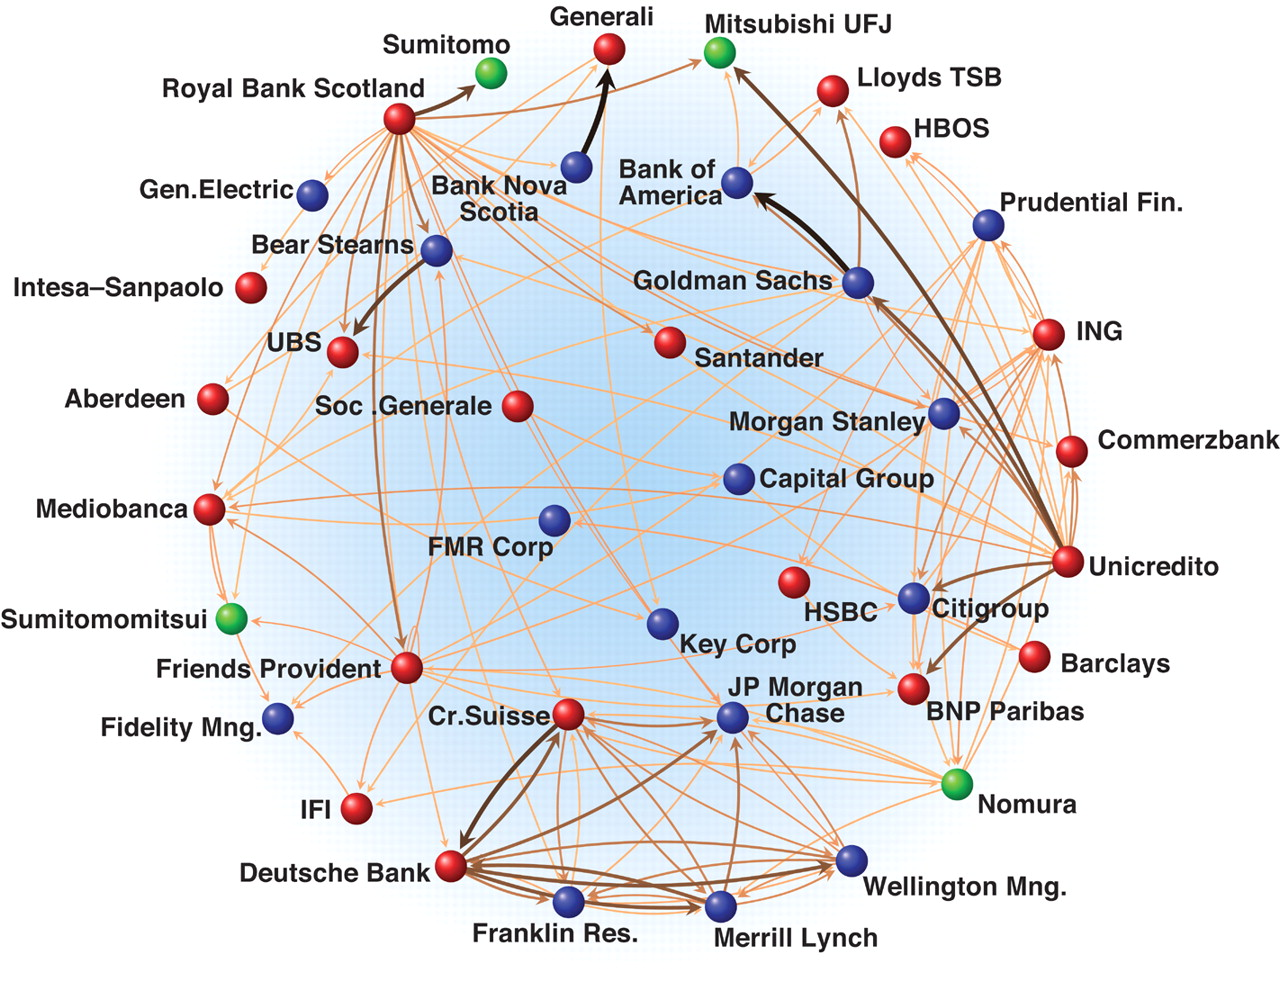
\includegraphics[width=0.5\textwidth]{bank_network.jpg}
		\caption{Bank Network}
		\cite[p. 424]{schweitzer2009economic}
		\label{fig:bank_network}
	\end{figure} 

	\noindent Modeling social interactions is another interesting application
	of graphs in the field of business \& economics. Social interactions can be
	modeled as social networks and provide valuable information for analyzing
	consumer behavior. This thesis will focus on gaining customer insights,
	which is an important and more business flavored application. Gaining
	customer insights has become an important topic and increasingly relies on
	graph machine learning. An example for this are social network companies 
	such as Facebook or search providers like Google. Those companies mainly 
	generate their revenue by providing customer insights or selling targeted 
	advertising to their clients \citep{Facebook2021,Alphabet2021}. Both 
	Facebook and Google have the advantage, that their businesses naturally 
	capture network- and feature data. It is for this reason, that these
	companies are ideally positioned to exploit the data on their platforms
	using graph machine learning. \\

	\noindent Most researchers and companies do not have access to datasets which
	include network information and feature data. In a practical setting,
	companies may have access to large amounts of customer data. This data
	however rarely contains any network information (e.g. which client is
	connect with which other clients). This scenario is similar for researchers
	and is especially true for social scientists which often have to collect 
	data via anonymous surveys. This makes the collection of network information 
	practically impossible. For that reason, companies and researchers are 
	typically confined to working with datasets which do not contain network 
	information. At this point it is important to mention, that there is a lot 
	of network data available online. This network data however typically does 
	not contain any feature data. This has the consequence, that researchers and 
	companies have to choose between network data or feature data. For the 
	purpose of gaining customer insights, feature data is more important. 
	Therefore, the most practical approach is to discard network information 
	and to focus on using feature data. This data access problem prevents many 
	researchers and companies to make use of potentially superior graph based 
	machine learning models. This problem motivates this master's thesis to find
	alternatives which at least in part remove the barrier for graph machine 
	learning. For that reason, alternative graph generation procedures are
	investigated and are presented along with the research topic in section 
	\ref{section:research_topics}. \\

	\noindent First, a general overview of the machine learning models used in
	this thesis is given in the following section.
	
	\section{Machine Learning Overview}

	This section provides a high-level overview of machine learning and
	specifies the type of machine learning task used in this thesis. To
	start, it is important to correctly categorize machine learning. There are
	many related big topics such as data science, big data or artificial
	intelligence and it is often not clear what exactly is meant. An overview
	of how these different terms can be categorized is shown in figure 
	\ref{fig:ml_overview}.

	\begin{figure}[h]
		\centering
		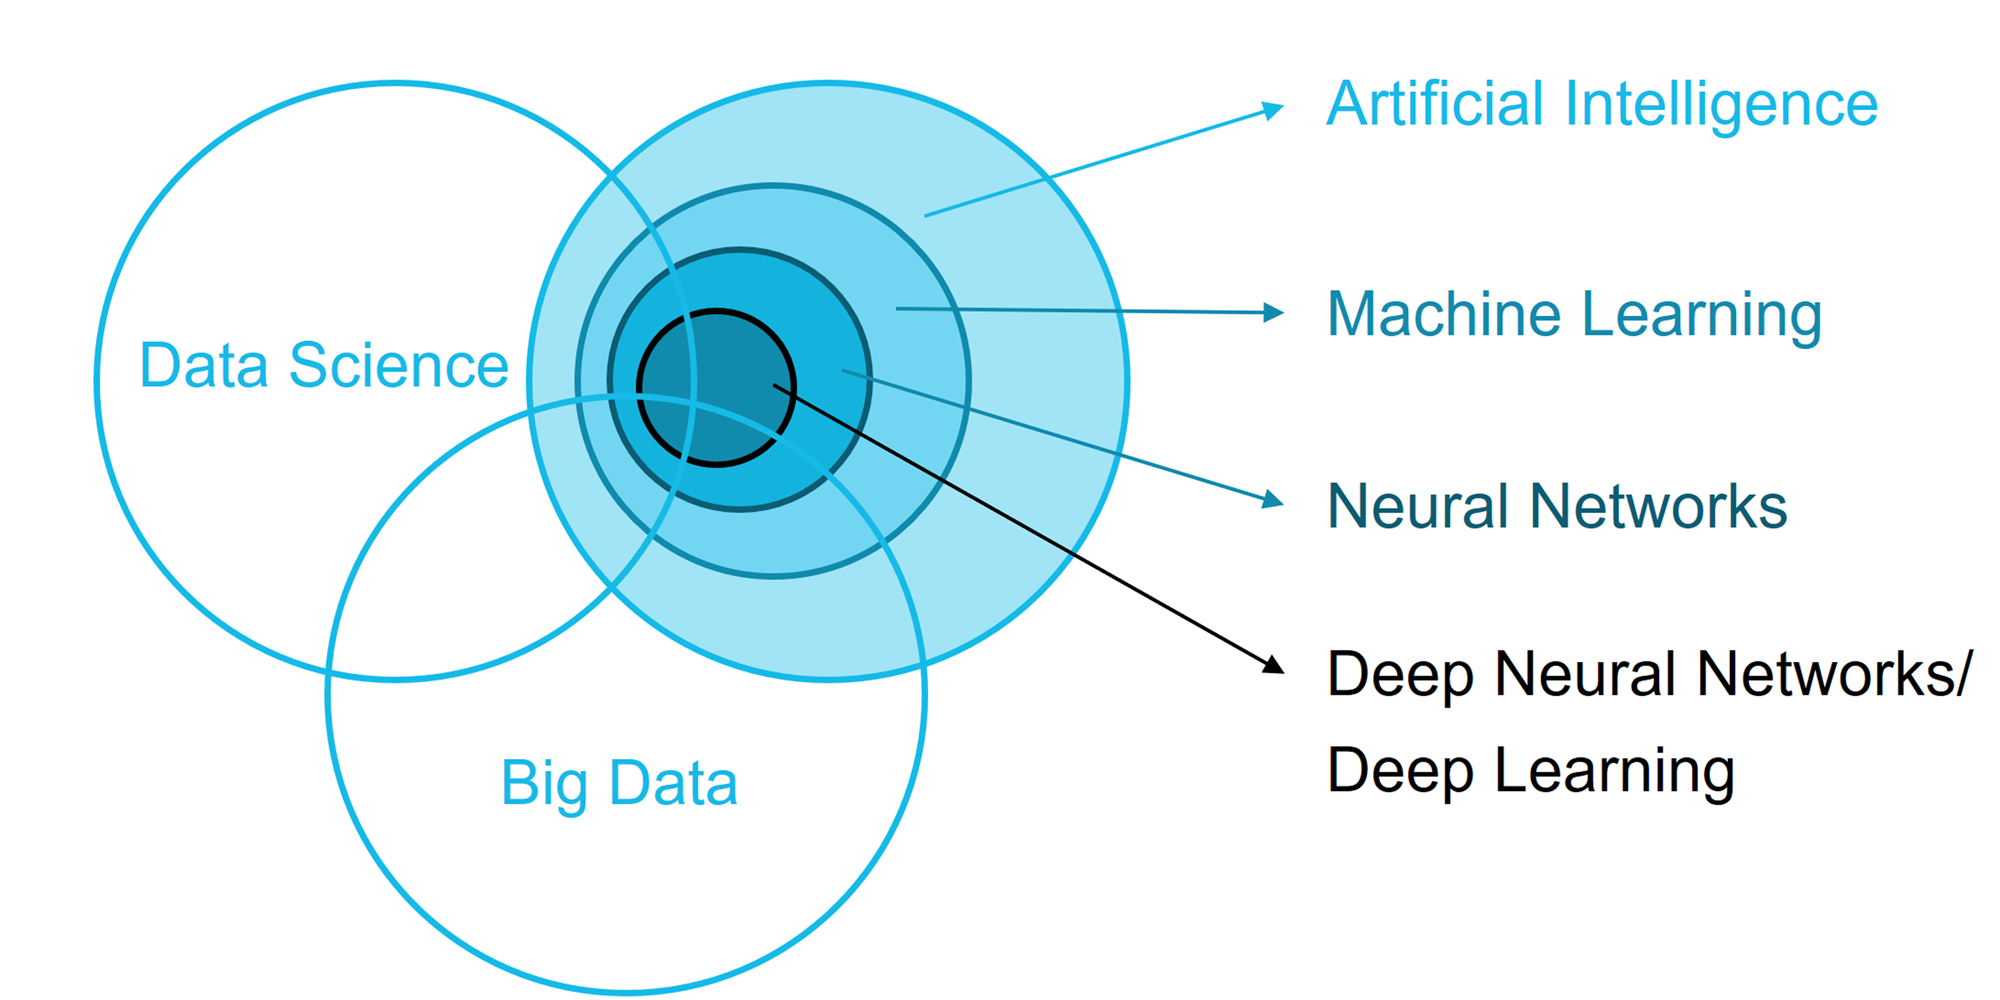
\includegraphics[width=0.7\textwidth]{overview_datascience.png}
		\caption{Machine Learning Overview}
		\citep{Frauenhofer2021}
		\label{fig:ml_overview}
	\end{figure} 

	\noindent Figure \ref{fig:ml_overview} depicts well, how these different
	terms are related with each other. Machine learning in particular is
	mostly ascribed to the domain of artificial intelligence. It however also 
	has a shared domain with data science and big data. It is thus at the
	intersection of these three interrelated fields. Machine learning models 
	such as neural networks and deep neural networks are specific models within
	machine learning and are often referred to separately due to their
	popularity. In this thesis, differentiating between machine learning and
	neural networks is not necessary, as the considered machine learning models
	are used for the same task. Machine learning can be applied for various
	tasks and is again best presented visually as shown in figure 
	\ref{fig:ml_tasks}.

	\begin{figure}[h]
		\centering
		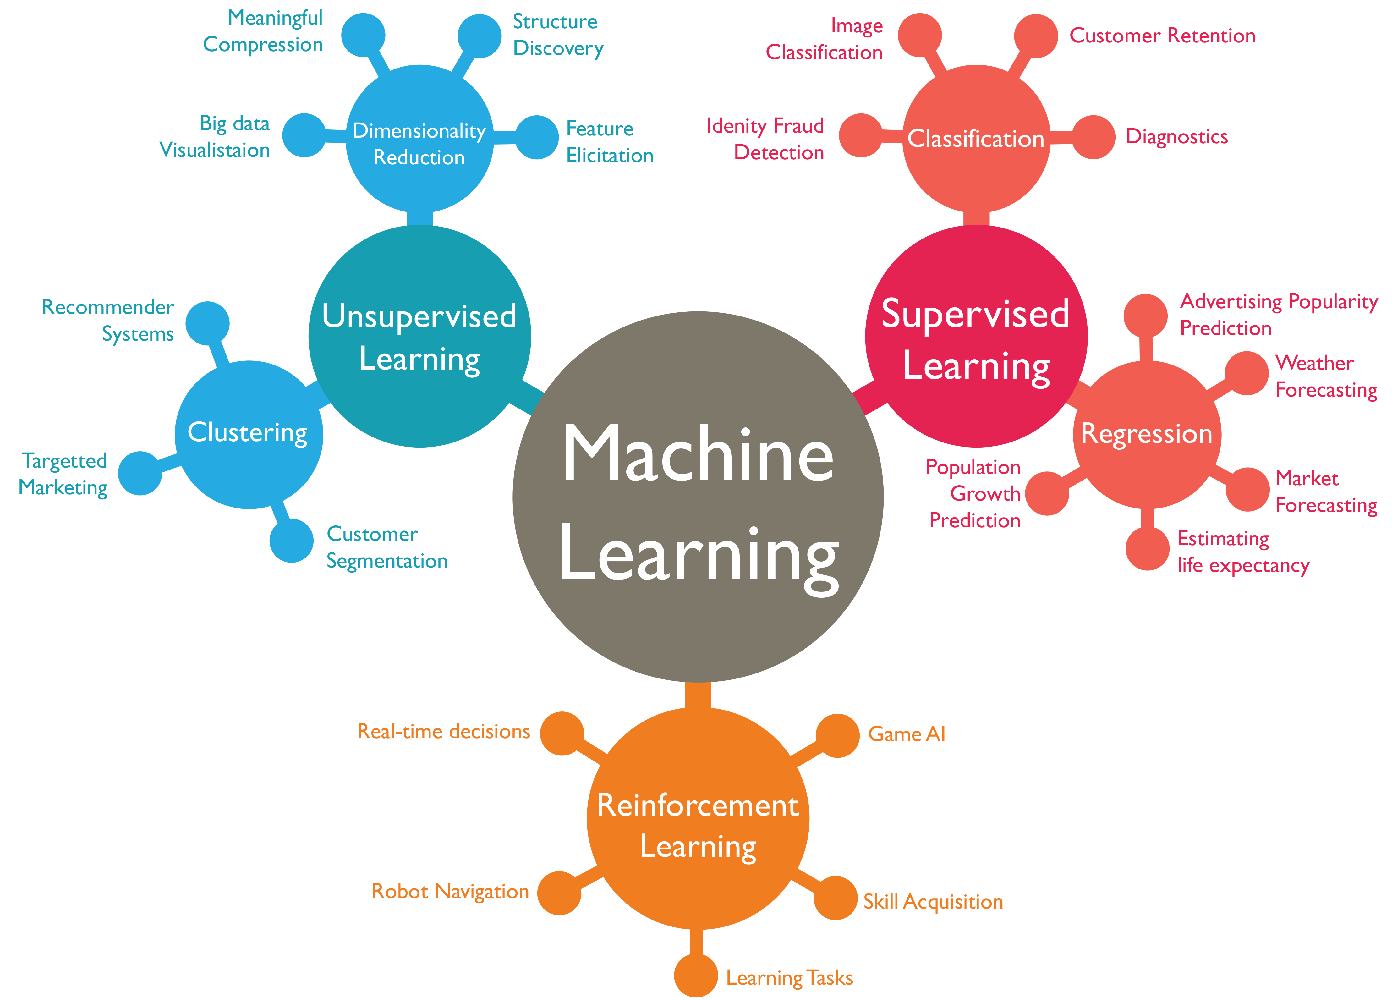
\includegraphics[width=0.8\textwidth]{ml_tasks.png}
		\caption{Overview Machine Learning Tasks}
		\citep{Artisan2020}
		\label{fig:ml_tasks}
	\end{figure} 

	\noindent It is shown in figure \ref{fig:ml_tasks}, that the main tasks for
	machine learning involve classification, regression, reinforcement
	learning, clustering and dimensionality reduction. This thesis focuses on 
	classification tasks. This task is chosen given the available data and 
	because it allows for a nice comparison of different machine learning models. 
	Well known standard machine learning models used for classification tasks 
	include logistic regression \citep{cramer2002origins}, naive bayes 
	\citep{zhang2004bayes}, \acp{svm} \citep{platt1999probabilistic}, 
	random forest classifiers \citep{breiman2001random}, AdaBoost 
	\citep{freund1997decision}, \ac{qda} \citep{tharwat2016linear} and 
	\acp{ann} \citep{mcculloch1943logical,werbos1974beyond}. This is an 
	incomplete list of popular machine learning models that can be used for 
	classification tasks. Well-known applications of classification tasks include 
	predicting whether a customer is satisfied, whether to grant a mortgage to 
	a client, and many more. The aforementioned machine learning models have in 
	common, that they can only consider feature data. It is in general not 
	possible to directly make use of network information for these models. \\

	\noindent Graph machine learning methods are special because they can 
	consider both feature data as well as network information. Using the
	overview shown in figure \ref{fig:ml_overview}, graph machine learning is
	probably best categorized as a special form of neural network. It is 
	however not a deep neural network, as network depth does not necessarily 
	improve the model and can be even counter-productive. Within graph machine 
	learning there are two main approaches. The first approach focuses on 
	learning vector representations of graphs which are then used for downstream 
	machine learning. The downstream machine learning models involve the standard 
	models presented previously. Graph representation learning approaches include 
	models such as DeepWalk \citep{perozzi2014deepwalk} and Node2Vec 
	\citep{grover2016node2vec} among others. The second approach involves the 
	application of \acp{gnn} for which there exist many different 
	models. Popular and established models include \acp{gcn}
	\citep{kipf2016semi} and GraphSage \citep{hamilton2017inductive}. The detailed 
	theoretical background for the considered graph machine learning models is 
	provided in chapter 2.

	\section{Research Topic}
	\label{section:research_topics}

	\noindent The difficult access to graphs which also contain features 
	motivates the search for alternatives. A review of the literature revealed, 
	that a form of synthetic graph generation could provide a solution to the data 
	access problem. Classic graph generation models include the famous 
	Erdös-Rényi graphs \citeyearpar{erdos1959random}, the small-world model by 
	\cite{watts1998collective}, the well-known model by 
	\cite{barabasi1999emergence}, and more recently Kronecker graphs by
	\cite{leskovec2010kronecker}. These models are all very instructive
	regarding the graph generation process and for understanding graph
	properties. These networks however all have the short-coming, that they do 
	not allow for the assignment of feature data to the nodes/observations in the
	network. It became clear, that one has to find or develop a model which 
	makes use of existing feature data for the graph generation process. 
	\cite{kim2012multiplicative} developed the \ac{mag} model. This model makes 
	use of randomly generated feature data which is referred to as attribute data 
	by the authors. The model is shown to be capable of generating random graphs 
	which can adhere to observed real world network properties. An analysis of 
	the \ac{mag} model revealed, that it could also be a useful model for 
	creating semi-synthetic graphs using existing feature data. For that reason, 
	the \acs{mag} model is selected for generating semi-synthetic graphs. This 
	model is introduced in detail in section \ref{section:theory_graphgen}. \\

	\noindent More recently, researchers have focused their attention on deep 
	generative graph models. These models create graphs with features using
	real graphs as a training input. Examples for such models are graph
	\aclp{rnn} \citep{you2018graphrnn} and deep generative graph
	models \citep{li2018learning}. These are very fascinating models which can
	be used to recreate or scale graph data. For the purpose of this thesis,
	these models are not useful as it requires an existing graph with
	features to be available. Such a graph was unfortunately not available for
	writing this master's thesis. Nevertheless, this is an interesting current 
	topic for graph generation which was considered. \\ 

	\noindent The \acs{mag} model is interesting as it could allow for the 
	creation of semi-synthetic graphs using feature data. Semi-synthetic refers
	to the fact, that the graph is generated using real feature data. A fully
	synthetic graph would be generated using completely artificial data. Many
	companies and researchers have access to large feature datasets. These
	datasets include customer databases or collected survey data. For that
	reason it would be of great benefit, if the \acs{mag} model could generate
	useful semi-synthetic graphs. The usefulness of a graph is determined to
	the extent, that the graph can be used for machine learning and yield a 
	high accuracy for a given classification task. It is not expected, that the 
	semi-synthetic graphs can fully substitute real graphs. Real world networks
	often capture connections, which are difficult to formalize and thus
	recreate using a model such as the \acs{mag}. Nevertheless, the
	semi-synthetic graphs could be capable of generating useful network
	information. If this holds true, the semi-synthetic graph contains richer
	data which can then be exploited using graph machine learning. To assess
	the viability of this approach, the results using semi-synthetic graphs
	should be able to outperform or at least compete with the results using
	standard machine learning models. Therefore to assess these hypotheses,
	the results using graph machine learning are compared to the results using 
	standard machine learning models. To close this section and chapter, the 
	research question as well as the hypotheses of this thesis are presented 
	formally as follows.
	\newpage
	\paragraph{Research Question}\mbox{}

	\noindent To what extent are semi-synthetic graphs based on real 
				feature data useful for a classification task using graph 
				machine learning?

	\paragraph{Hypotheses}\mbox{}

	\noindent\textbf{H1:} Graph machine learning using semi-synthetic graphs
	provide superior results compared to the results of standard machine
	learning for a given classification task.\\

	\noindent\textbf{H2:} Graph machine learning using semi-synthetic graphs is
	a competitive strategy compared to the results of standard machine
	learning for a given classification task.\\

